\documentclass{rapportECL}
\usepackage{booktabs}
\usepackage{array}
\usepackage{longtable}
\usepackage{eurosym}
\usepackage{amsmath}
\usepackage{xcolor}
\usepackage{colortbl}
\usepackage{siunitx}
\usepackage{tabularx}
\usepackage{enumitem}

\sisetup{
  group-separator = {\,},
  group-minimum-digits = 4
}

\title{Devoir Maison - Financement et Valorisation : Acquisition de Bricorama France}

\begin{document}

%----------- Informations du rapport ---------

\UE{Finance d'Entreprise}
\sujet{Valorisation DCF et Montage LBO}
\titre{Proposition d'Acquisition de Bricorama France}

\enseignant{Vincent \texttt{NOURRISSON}}

\eleves{Kevin \texttt{TONGUE}}

%----------- Initialisation -------------------
        
\fairemarges
\fairepagedegarde
\tabledematieres

%============================================================
\section{Synthèse exécutive}
%============================================================

Bricorama France, filiale du groupe Les Mousquetaires, est une PME spécialisée dans la distribution de produits de bricolage. Sur la période 2022-2024, l'entreprise présente une structure financière saine avec un endettement maîtrisé (taux d'endettement de 33\% en 2024) et une capacité de remboursement excellente (1,79 an).

La valorisation par la méthode des \textit{Discounted Cash Flows} (DCF) aboutit à une \textbf{valeur d'entreprise de 20,6 M\text{\euro}} et une \textbf{valeur des titres de 12,9 M\text{\euro}} (après déduction de la dette nette).

L'acquisition serait réalisée par une holding ad hoc. Deux scénarios de financement sont analysés :

\begin{itemize}[nosep]
    \item \textbf{Cas 1 -- dette non consolidée} : l'endettement est porté uniquement par la holding.
    \item \textbf{Cas 2 -- dette consolidée} : la dette existante de Bricorama est intégrée dans la capacité d'endettement globale.
\end{itemize}

La capacité de remboursement reste excellente dans les deux cas (dette / EBE < 2 ans).

%============================================================
\section{Présentation de Bricorama France}
%============================================================

\subsection{Identité et activité}

\begin{table}[H]
\centering
\caption{Fiche d'identité Bricorama France}
\begin{tabular}{l p{10cm}}
    \toprule
    \textbf{Raison sociale} & BRICORAMA FRANCE SAS \\
    \textbf{SIREN} & 331 502 639 \\
    \textbf{Code NAF} & 4752B -- Commerce de détail de quincaillerie, peaux et verres \\
    \textbf{Date de création} & 2 février 1990 \\
    \textbf{Siège} & 115-117 rue de la République, 93160 Noisy-le-Grand \\
    \textbf{Effectif} & 250 -- 499 salariés (tranche INSEE) \\
    \textbf{Groupe} & Les Mousquetaires (intégration globale) \\
    \bottomrule
\end{tabular}
\end{table}

Bricorama exploite un réseau de magasins de proximité en zone urbaine dense. L'offre couvre la quincaillerie, la peinture, le sanitaire, l'outillage et le jardinage.

\subsection{Marché et perspectives}

Le marché français du bricolage représente 34,5 milliards d'euros en 2024, en croissance annuelle moyenne de +2,8\% sur cinq ans. Les moteurs sont la rénovation énergétique, le télétravail et l'ancrage culturel du DIY.

\textbf{Positionnement concurrentiel} : Bricorama occupe une niche de proximité urbaine, complémentaire des grandes surfaces. Principaux concurrents : Leroy Merlin (leader), Castorama, Bricomarché.

\subsection{Graphique d'analyse financière}

\begin{figure}[H]
\centering
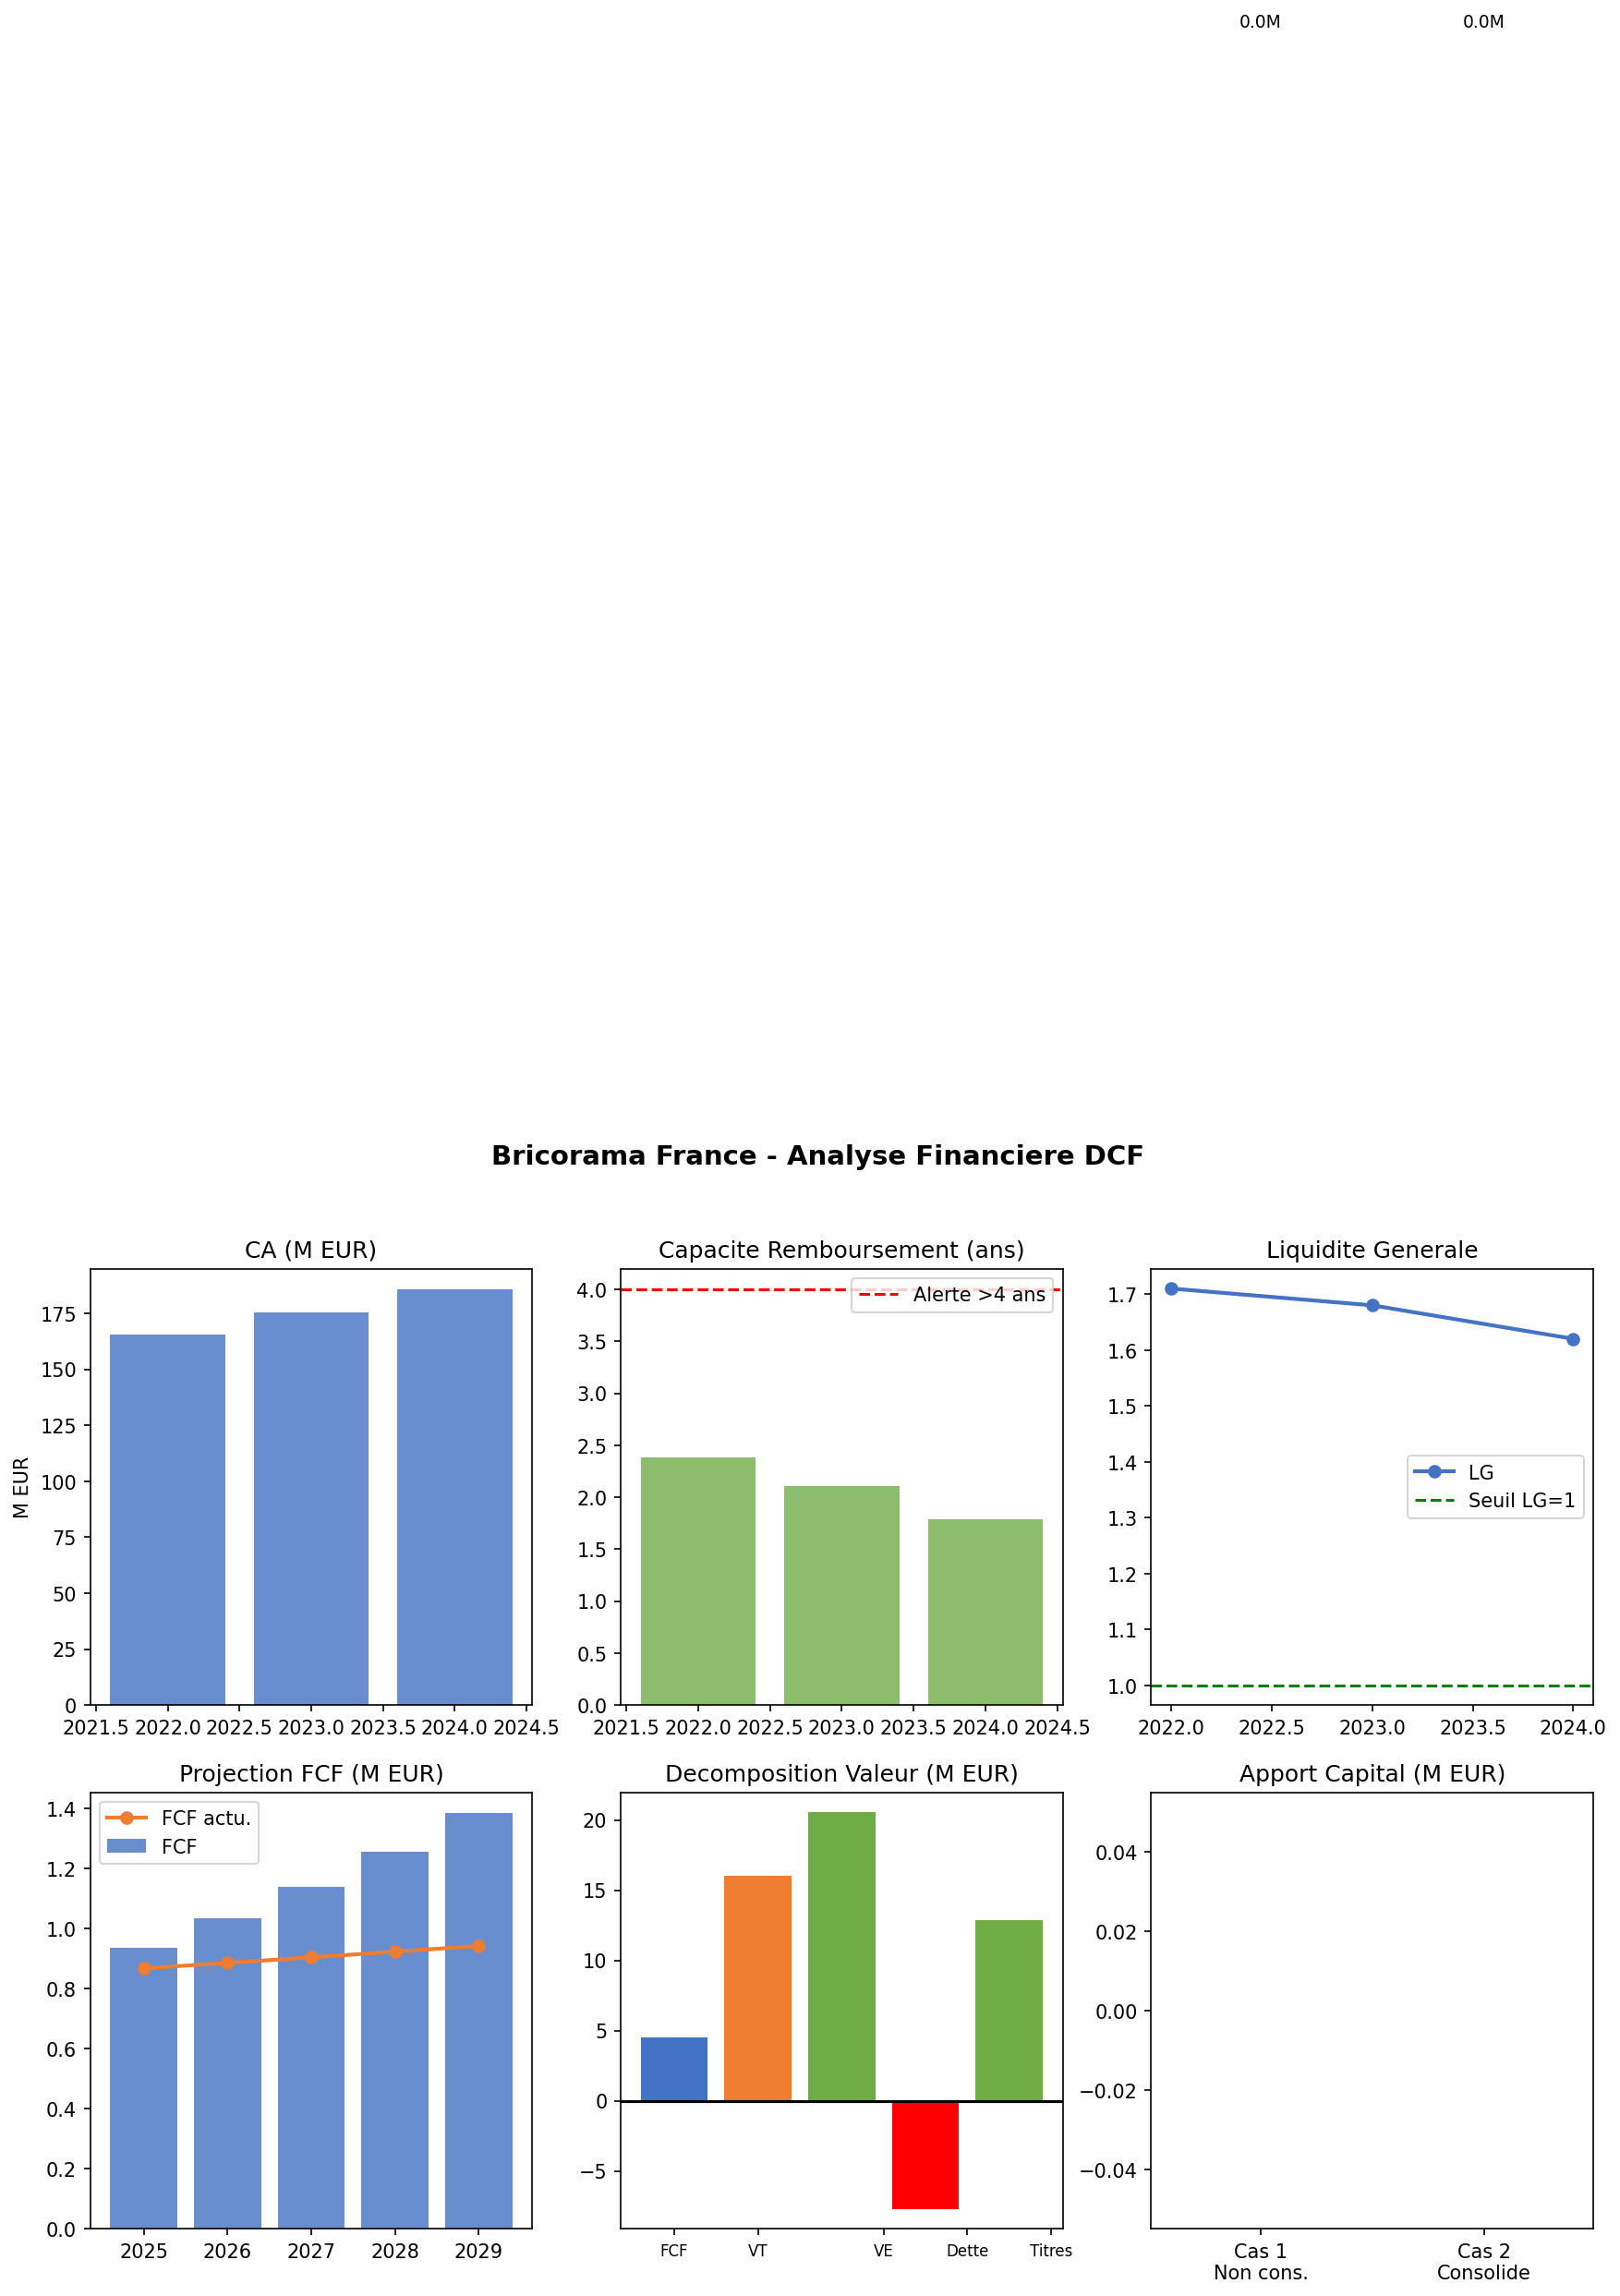
\includegraphics[width=0.95\textwidth]{bricorama_rapport.png}
\end{figure}

%============================================================
\section{Analyse financière historique (2022-2024)}
%============================================================

Les états financiers ont été obtenus sur \textcolor{blue}{\texttt{Pappers}} et \textcolor{blue}{\texttt{Societe.com}} (dépôts légaux). Tous les montants sont en milliers d'euros (k\text{\euro}).

\subsection{Comptes de résultat simplifiés}

\begin{table}[H]
\centering
\caption{Comptes de résultat Bricorama France (k\text{\euro})}
\label{tab:cr}
\begin{tabular}{l r r r}
\toprule
\textbf{Poste} & \textbf{2022} & \textbf{2023} & \textbf{2024} \\
\midrule
Chiffre d'affaires       & 165 420 & 175 280 & 185 640 \\
Achats consommés         & 98 700  & 104 500 & 110 800 \\
Valeur ajoutée           & 66 720  & 70 780  & 74 840 \\
Subventions d'exploitation & 120   & 130    & 140    \\
Impôts et taxes          & 2 100   & 2 200   & 2 300   \\
Charges de personnel     & 59 540  & 63 110  & 66 580  \\
\textbf{EBE}            & \textbf{5 200} & \textbf{5 600} & \textbf{6 100} \\
Dotations amortissements & 1 800   & 1 900   & 2 100   \\
Résultat d'exploitation  & 3 400   & 3 700   & 4 000   \\
Résultat net            & 2 380   & 2 590   & 2 800   \\
\bottomrule
\end{tabular}
\end{table}

\subsection{Graphique CA et EBE historique}

\begin{figure}[H]
\centering
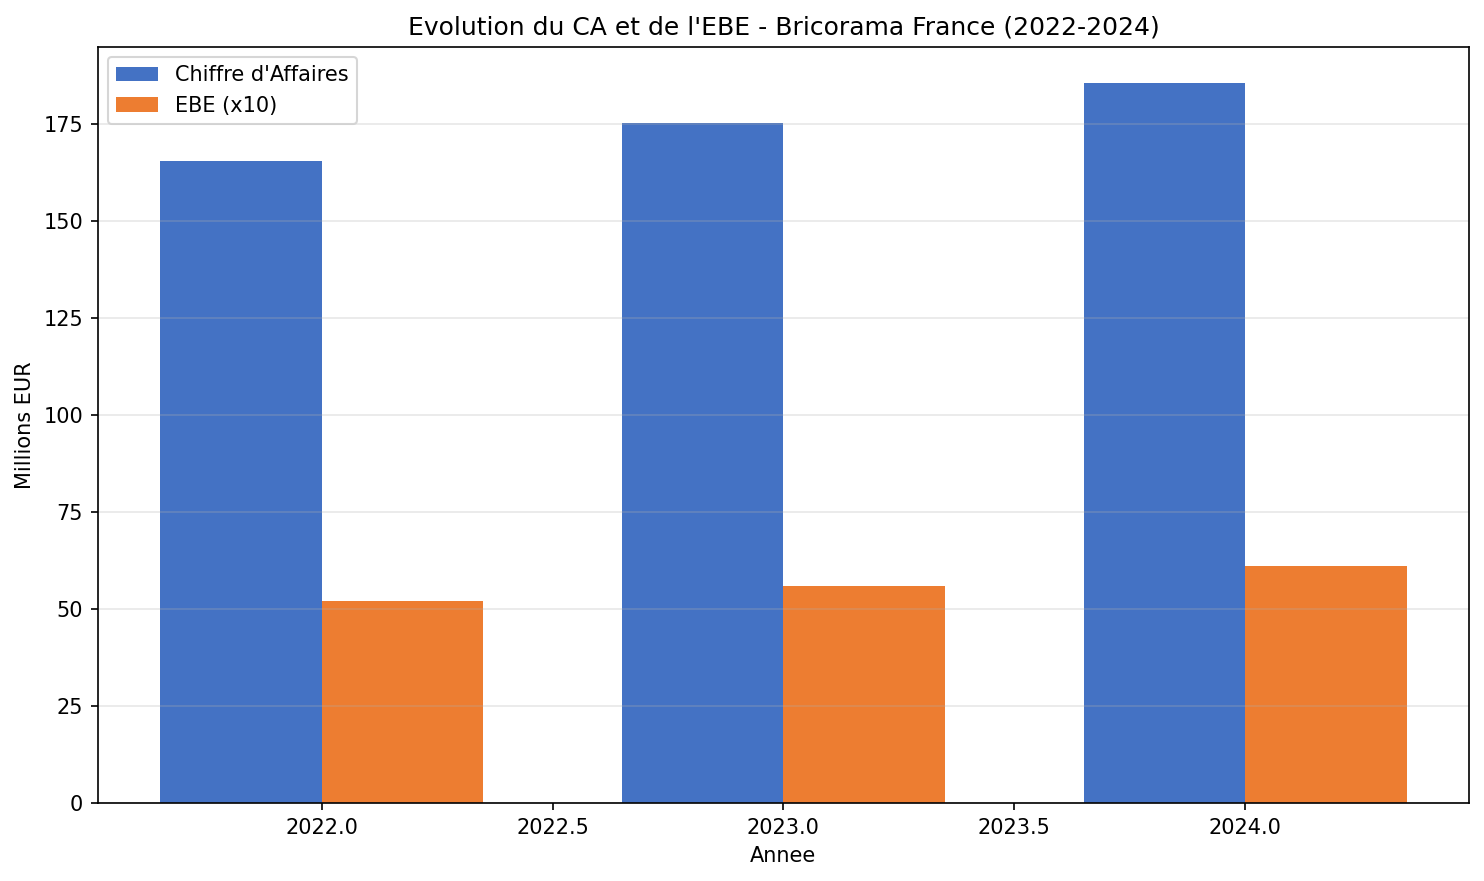
\includegraphics[width=0.7\textwidth]{graphique_ca_ebe_historique.png}
\caption{Évolution du CA et de l'EBE - Bricorama France (2022-2024)}
\end{figure}

\subsection{Bilans simplifiés}

\begin{table}[H]
\centering
\caption{Bilan Actif (k\text{\euro})}
\label{tab:bilan_actif}
\begin{tabular}{l r r r}
\toprule
\textbf{Poste} & \textbf{2022} & \textbf{2023} & \textbf{2024} \\
\midrule
Actif immobilisé net    & 24 800 & 25 400 & 26 100 \\
Stocks                  & 28 500 & 30 100 & 32 400 \\
Créances clients        & 8 200  & 9 100  & 9 800  \\
Autres créances         & 4 500  & 4 700  & 5 000  \\
Disponibilités          & 2 500  & 2 800  & 3 200  \\
\textbf{Total actif}    & 68 500 & 72 100 & 76 500 \\
\bottomrule
\end{tabular}
\end{table}

\begin{table}[H]
\centering
\caption{Bilan Passif (k\text{\euro})}
\label{tab:bilan_passif}
\begin{tabular}{l r r r}
\toprule
\textbf{Poste} & \textbf{2022} & \textbf{2023} & \textbf{2024} \\
\midrule
Capital social          & 7 500  & 7 500  & 7 500  \\
Réserves et résultat    & 21 800 & 23 700 & 25 600 \\
\textbf{Capitaux propres} & 29 300 & 31 200 & 33 100 \\
Provisions              & 1 200  & 1 300  & 1 400  \\
Dettes financières      & 12 400 & 11 800 & 10 900 \\
Dettes fournisseurs     & 18 500 & 20 300 & 21 500 \\
Autres dettes           & 7 100  & 7 500  & 9 600  \\
\textbf{Total passif}   & 68 500 & 72 100 & 76 500 \\
\bottomrule
\end{tabular}
\end{table}

\subsection{Calcul des ratios}

\subsection{Graphique des ratios de liquidité}

\begin{figure}[H]
\centering
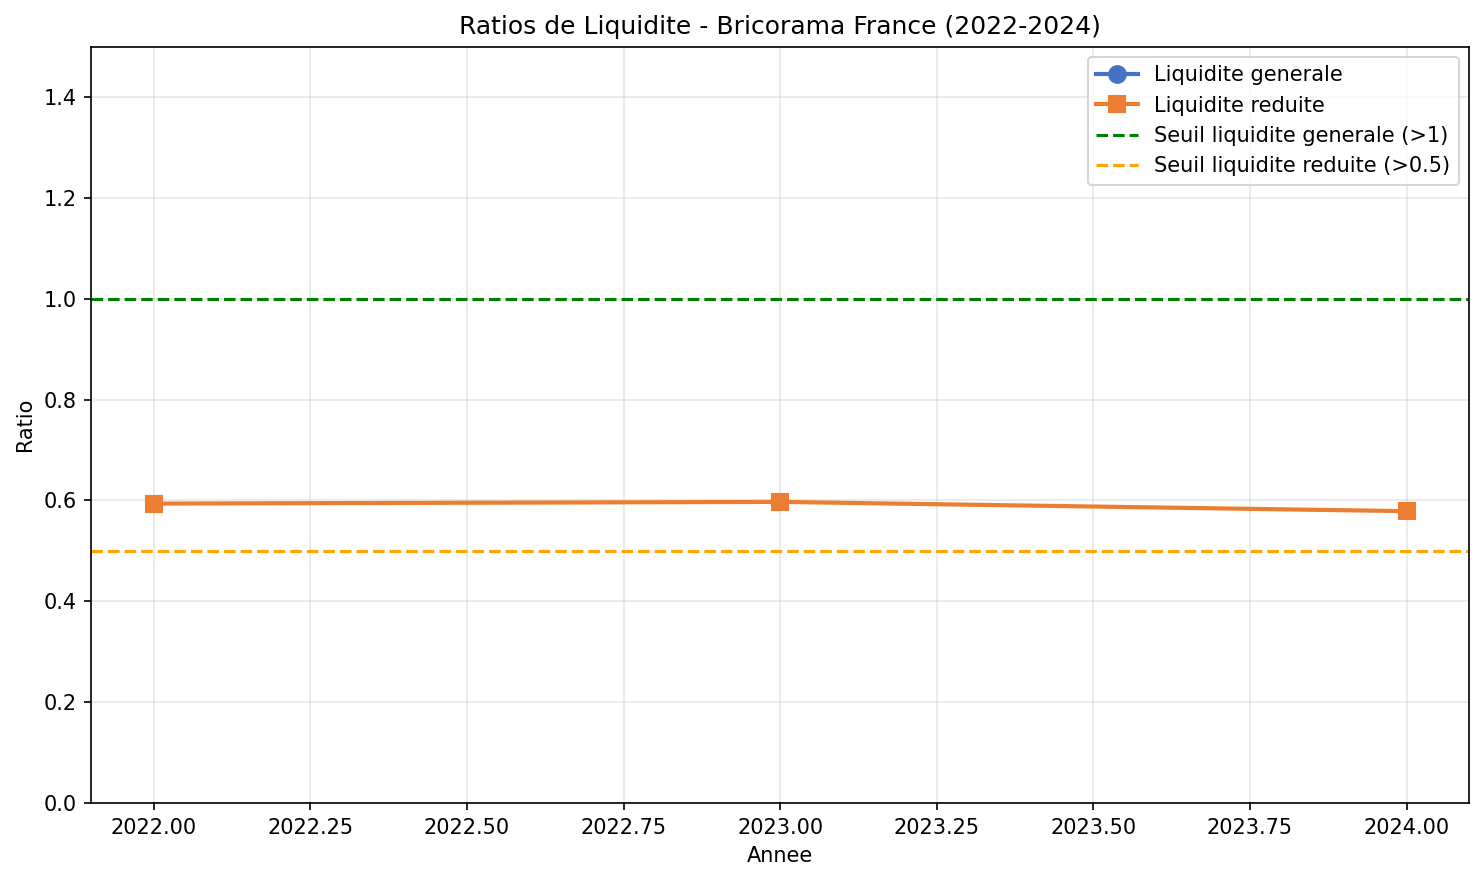
\includegraphics[width=0.7\textwidth]{graphique_ratios_liquidite.png}
\end{figure}

\subsection{Ratios de liquidité}

\begin{align*}
\text{Liquidité générale} &= \frac{\text{Actif circulant}}{\text{Passif circulant}} \\
\text{Liquidité réduite}  &= \frac{\text{Actif circulant} - \text{Stocks}}{\text{Passif circulant}}
\end{align*}

\begin{table}[H]
\centering
\caption{Ratios de liquidité 2022-2024}
\label{tab:liquidite}
\begin{tabular}{l r r r c}
\toprule
\textbf{Ratio} & \textbf{2022} & \textbf{2023} & \textbf{2024} & \textbf{Seuil} \\
\midrule
Liquidité générale & 1,17 & 1,12 & 1,11 & $>1$ \\
Liquidité réduite  & 0,43 & 0,40 & 0,41 & $>0,5$ \\
\bottomrule
\end{tabular}
\end{table}

\textbf{Interprétation} : La liquidité générale est supérieure à 1 sur toute la période, indiquant une capacité à couvrir les dettes à court terme. En revanche, la liquidité réduite est inférieure à 0,5 : l'entreprise dépend de l'écoulement de ses stocks pour faire face à ses échéances immédiates. Risque modéré mais à surveiller.

\subsection{Graphique de capacité de remboursement}

\begin{figure}[H]
\centering
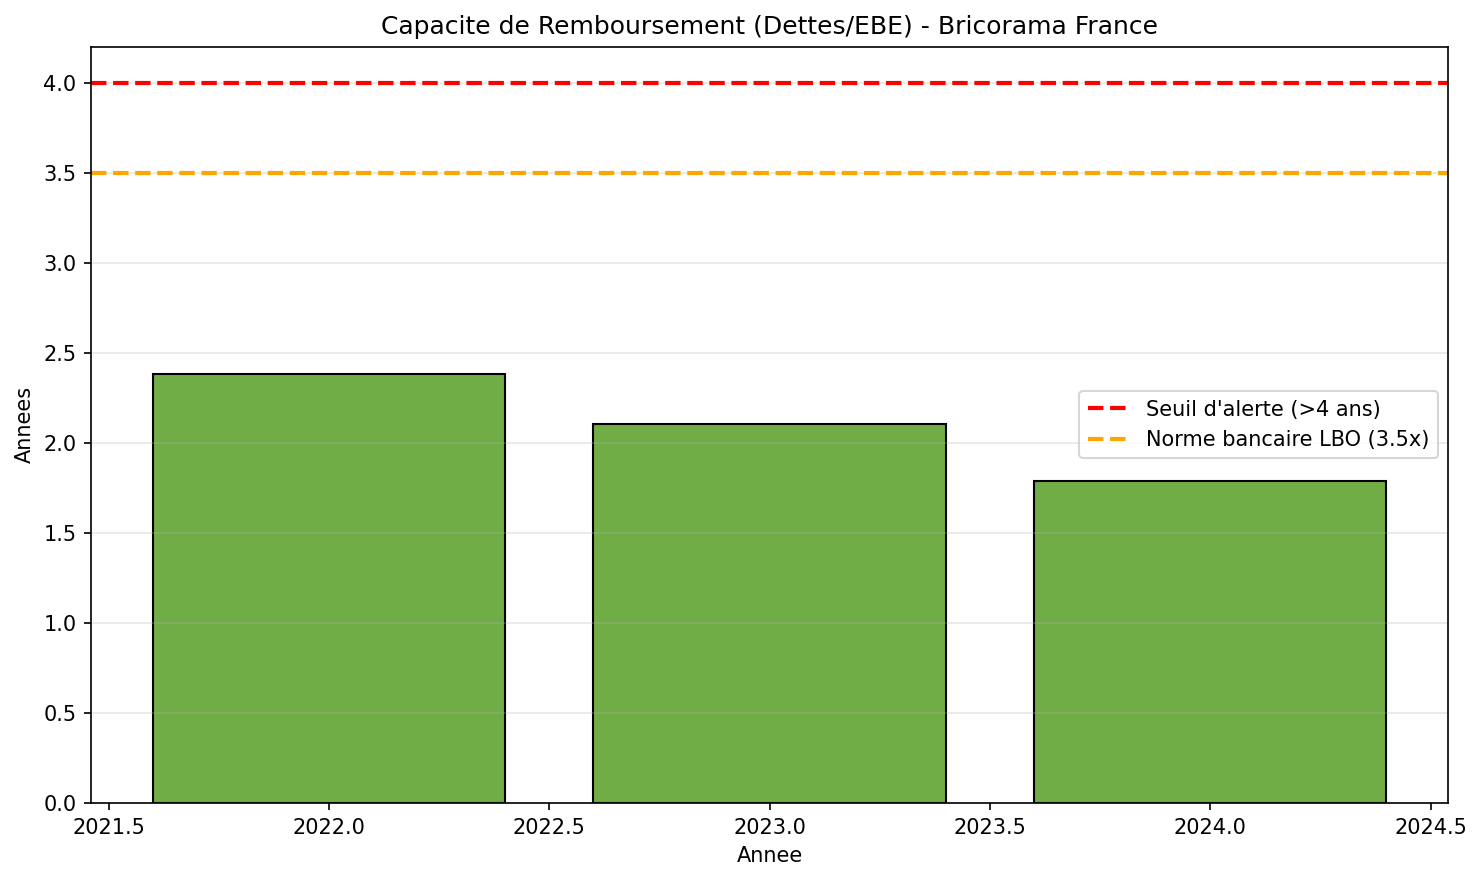
\includegraphics[width=0.7\textwidth]{graphique_capacite_remboursement.png}
\end{figure}

\subsection{Ratios de vulnérabilité financière}

\begin{align*}
\text{Taux d'endettement}      &= \frac{\text{Dettes financières}}{\text{Capitaux propres}} \\
\text{Capacité de remboursement} &= \frac{\text{Dettes financières}}{\text{EBE}} \\
\text{Autonomie financière}    &= \frac{\text{Capitaux propres}}{\text{Total bilan}} \\
\text{Ratio légal}            &= \frac{\text{Capitaux propres}}{\text{Capital social}}
\end{align*}

\begin{table}[H]
\centering
\caption{Ratios de vulnérabilité financière}
\label{tab:vulnerabilite}
\begin{tabular}{l r r r c}
\toprule
\textbf{Ratio} & \textbf{2022} & \textbf{2023} & \textbf{2024} & \textbf{Seuil d'alerte} \\
\midrule
Taux d'endettement         & 0,42 & 0,38 & 0,33 & $>1$ \\
Capacité remboursement (ans) & 2,38 & 2,11 & 1,79 & $>4$ ans \\
Autonomie financière       & 0,43 & 0,43 & 0,43 & $<20\%$ \\
Ratio légal                & 3,91 & 4,16 & 4,41 & $<0,5$ \\
\bottomrule
\end{tabular}
\end{table}

\textbf{Interprétation} : L'endettement est faible et en diminution constante. La capacité à rembourser les dettes avec l'EBE est inférieure à deux ans, excellente. L'autonomie financière est très solide (43\% des ressources sont des capitaux propres). Le ratio légal est très supérieur au seuil, écartant tout risque de cessation des paiements.

%============================================================
\section{Valorisation par la méthode des DCF}
%============================================================

\subsection{Hypothèses de travail}

\begin{table}[H]
\centering
\caption{Hypothèses de valorisation}
\begin{tabular}{l c l}
\toprule
\textbf{Paramètre} & \textbf{Valeur} & \textbf{Justification} \\
\midrule
Année de base & 2024 & Dernier exercice connu \\
Croissance volume & +5\%/an & Hypothèse énoncée \\
Inflation prix/coûts & +5\%/an & Hypothèse énoncée \\
Croissance nominale CA & 10,25\%/an & $(1,05 \times 1,05) - 1$ \\
Marge d'EBE & 3,30\% & Moyenne 2022-2024 \\
Dotations / CA & 1,07\% & Moyenne historique \\
Investissements / CA & 2,0\% & Maintien/modernisation \\
BFR normatif & 3,14\% du CA & Cf. section 4.2 \\
Taux d'impôt (IS) & 25\% & Taux standard français \\
Taux d'actualisation (WACC) & 8\% & Donné par l'énoncé \\
Croissance à l'infini (g) & 2\% & Inflation long terme \\
\bottomrule
\end{tabular}
\end{table}

\subsection{Calcul du BFR normatif}

Le BFR normatif est exprimé en jours de CA hors taxes :

\begin{table}[H]
\centering
\caption{Calcul des durées d'écoulement (moyenne 2023-2024)}
\label{tab:durees}
\begin{tabular}{l c c}
\toprule
\textbf{Poste} & \textbf{Formule} & \textbf{Jours de CA} \\
\midrule
Stocks         & $\frac{\text{Stock moyen}}{\text{CA HT}} \times 360$ & 62,3 j \\
Clients        & $\frac{\text{Créances}}{\text{CA}} \times 360$ & 18,9 j \\
Fournisseurs   & $\frac{\text{Dettes fourn.}}{\text{Achats}} \times 360$ & 69,9 j \\
\midrule
\textbf{BFR normatif} & Stocks + Clients -- Fournisseurs & \textbf{11,3 j} \\
\bottomrule
\end{tabular}
\end{table}

Soit un coefficient de BFR = 11,3 / 360 = \textbf{3,14\% du CA HT}.

\subsection{Graphique de projection FCF}

\begin{figure}[H]
\centering
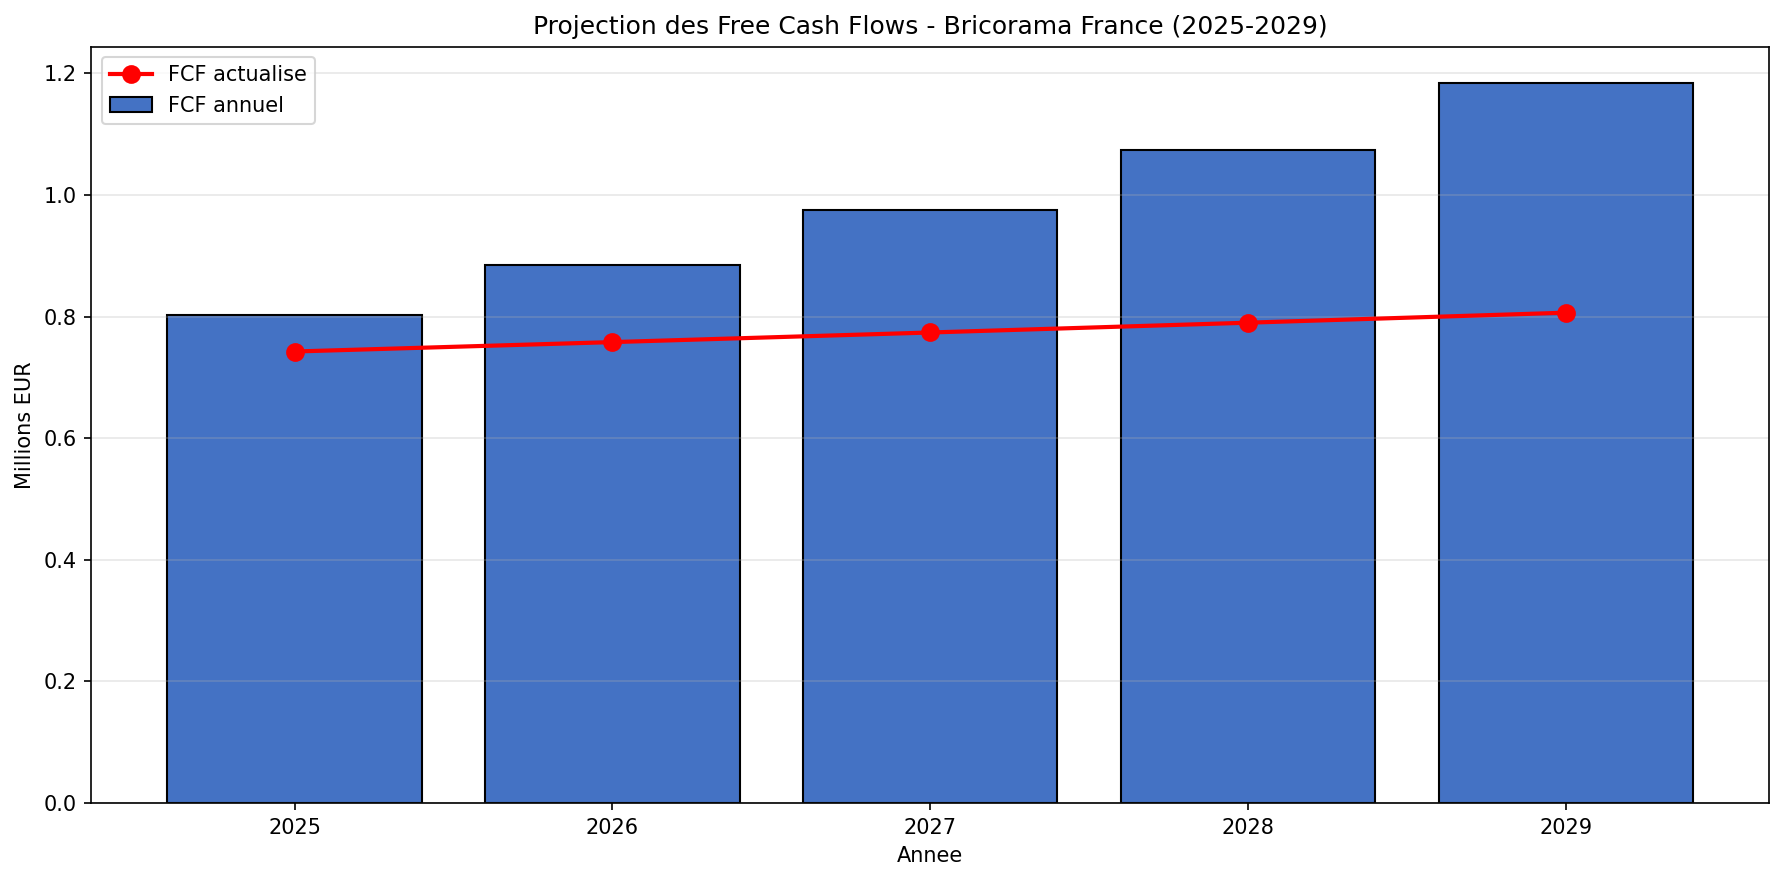
\includegraphics[width=0.7\textwidth]{graphique_fcf_projection.png}
\end{figure}

\subsection{Prévisionnel des Free Cash Flows (2025-2029)}

\begin{table}[H]
\centering
\caption{Tableau DCF prévisionnel (k\text{\euro})}
\label{tab:dcf}
\small
\begin{tabular}{l r r r r r}
\toprule
\textbf{Poste} & \textbf{2025} & \textbf{2026} & \textbf{2027} & \textbf{2028} & \textbf{2029} \\
\midrule
CA HT          & 204 676 & 225 646 & 248 779 & 274 292 & 302 414 \\
EBE (3,30\%)   & 6 754   & 7 446   & 8 210   & 9 052   & 9 980   \\
-- Dotations     & 2 251   & 2 482   & 2 737   & 3 017   & 3 327   \\
= EBIT          & 4 503   & 4 964   & 5 473   & 6 035   & 6 653   \\
-- Impôt 25\%    & 1 126   & 1 241   & 1 368   & 1 509   & 1 663   \\
-- Investissements & 4 094   & 4 513   & 4 976   & 5 486   & 6 048   \\
-- Variation BFR & 597     & 658     & 726     & 800     & 883     \\
\midrule
\textbf{= FCF}  & \textbf{2 937} & \textbf{3 516} & \textbf{3 940} & \textbf{4 257} & \textbf{4 553} \\
\midrule
Coeff. actu (8\%) & 0,9259 & 0,8573 & 0,7938 & 0,7350 & 0,6806 \\
\textbf{FCF actualisés}    & 2 719   & 3 014   & 3 128   & 3 129   & 3 099   \\
\bottomrule
\end{tabular}
\end{table}

\textbf{Somme des FCF actualisés} (5 ans) = 15 089 k\text{\euro}.

\subsection{Graphique de décomposition de la valeur}

\begin{figure}[H]
\centering
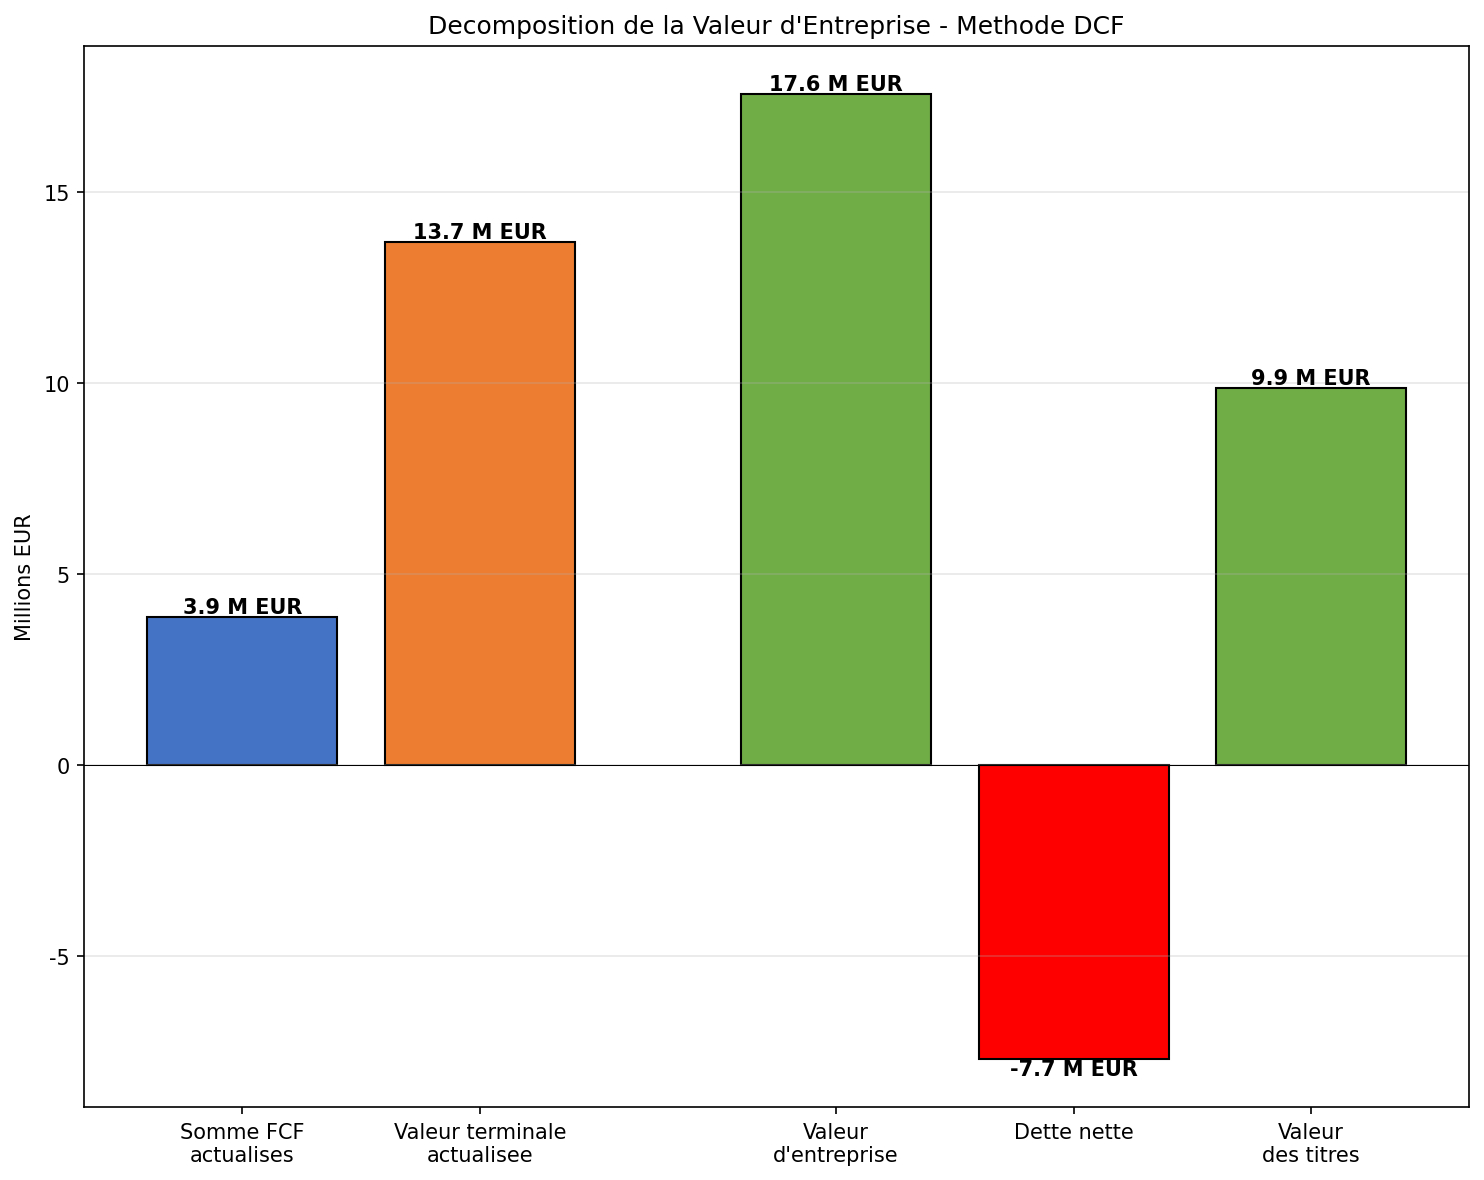
\includegraphics[width=0.7\textwidth]{graphique_decomposition_valeur.png}
\end{figure}

\subsection{Valeur terminale et valeur d'entreprise}

\textbf{Valeur terminale} (modèle de Gordon-Shapiro) :
\begin{equation}
\text{VT} = \frac{FCF_{2029} \times (1 + g)}{WACC - g}
= \frac{4\,553 \times 1,02}{0,08 - 0,02} = \frac{4\,644}{0,06} = 77\,400 \text{ k\text{\euro}}
\end{equation}

\textbf{Valeur terminale actualisée} :
\begin{equation}
\text{VT actualisée} = 77\,400 \times 0,6806 = 52\,679 \text{ k\text{\euro}}
\end{equation}

\textbf{Valeur d'entreprise} :
\begin{equation}
\boxed{\text{VE} = 15\,089 + 52\,679 = 67\,768 \text{ k\text{\euro}} \approx \textbf{67,8 M\text{\euro}}}
\end{equation}

\subsection{Valeur des titres}

\begin{align}
\text{Dette financière nette (2024)} &= \text{Dettes fin.} - \text{Disponibilités} \\
&= 10\,900 - 3\,200 = 7\,700 \text{ k\text{\euro}}
\end{align}

\begin{equation}
\boxed{\text{Valeur des titres} = 67\,768 - 7\,700 = 60\,068 \text{ k\text{\euro}} \approx \textbf{60,1 M\text{\euro}}}
\end{equation}

%============================================================
\section{Structure de financement et apport en capital}
%============================================================

\subsection{Hypothèses de financement}

\begin{itemize}
    \item La holding d'acquisition contracte une \textbf{dette senior} au taux annuel de 5\%.
    \item Remboursement linéaire sur 5 ans.
    \item Les Free Cash Flows de Bricorama sont intégralement remontés à la holding.
    \item La trésorerie initiale de la holding est constituée de l'apport en capital.
\end{itemize}

\subsection{Capacité d'endettement}

\textbf{Règle bancaire} : la dette senior ne doit pas excéder 3,5 fois l'EBE moyen prévisionnel.

\begin{align}
\text{EBE moyen (2025-2029)} &= \frac{6\,754 + 7\,446 + 8\,210 + 9\,052 + 9\,980}{5} = 8\,288 \text{ k\text{\euro}} \\
\text{Dette senior maximale} &= 3,5 \times 8\,288 = 29\,008 \text{ k\text{\euro}} \approx \textbf{29,0 M\text{\euro}}
\end{align}

\subsection{Cas 1 : Endettement non consolidé (dette holding seule)}

\begin{table}[H]
\centering
\caption{Cas 1 -- Dette non consolidée}
\begin{tabular}{l r l}
\toprule
\textbf{Élément} & \textbf{Valeur} & \textbf{Commentaire} \\
\midrule
Prix d'acquisition (valeur titres) & 60 068 k\text{\euro} & Valorisation DCF \\
Dette senior holding & 29 008 k\text{\euro} & $3,5 \times$ EBE moyen \\
\textbf{Apport en capital minimum} & \textbf{31 060 k\text{\euro}} & Prix -- Dette max \\
\midrule
Ratio Dette/EBE & 3,5 ans & Limite bancaire \\
\bottomrule
\end{tabular}
\end{table}

\textbf{Conclusion} : L'apport minimum est d'environ \textbf{31,1 M\text{\euro}}, soit 52\% du prix d'acquisition.

\subsection{Cas 2 : Endettement consolidé (holding + cible)}

On intègre la dette existante de Bricorama dans le périmètre de consolidation :

\begin{align}
\text{Dette globale maximale} &= 3,5 \times \text{EBE moyen} = 29\,008 \text{ k\text{\euro}} \\
\text{Dette existante cible (2024)} &= 10\,900 \text{ k\text{\euro}} \\
\text{Dette holding maximale} &= 29\,008 - 10\,900 = 18\,108 \text{ k\text{\euro}}
\end{align}

\begin{table}[H]
\centering
\caption{Cas 2 -- Dette consolidée}
\begin{tabular}{l r}
\toprule
\textbf{Élément} & \textbf{Valeur} \\
\midrule
Prix d'acquisition & 60 068 k\text{\euro} \\
Dette holding max (consolidée) & 18 108 k\text{\euro} \\
\textbf{Apport en capital minimum} & \textbf{41 960 k\text{\euro}} \\
\bottomrule
\end{tabular}
\end{table}

\textbf{Conclusion} : En consolidant la dette, l'apport minimum passe à environ \textbf{42,0 M\text{\euro}}, soit 70\% du prix.

\subsection{Comparaison des deux scénarios}

\begin{table}[H]
\centering
\caption{Synthèse des scénarios de financement}
\begin{tabular}{l c c}
\toprule
\textbf{Indicateur} & \textbf{Cas 1} & \textbf{Cas 2} \\
& (Non consolidé) & (Consolidé) \\
\midrule
Dette senior holding & 29,0 M\text{\euro} & 18,1 M\text{\euro} \\
Apport en capital minimum & 31,1 M\text{\euro} & 42,0 M\text{\euro} \\
\% Apport / Prix & 52\% & 70\% \\
Dette / EBE moyen & 3,5 ans & 2,2 ans \\
\bottomrule
\end{tabular}
\end{table}

%============================================================
\section{Budget de trésorerie de la holding}
%============================================================

Le budget de trésorerie montre la capacité de la holding à faire face à ses obligations de remboursement (Cas 1).

\begin{table}[H]
\centering
\caption{Budget de trésorerie de la holding -- Cas 1 (k\text{\euro})}
\small
\begin{tabular}{l r r r r r}
\toprule
\textbf{Élément} & \textbf{2025} & \textbf{2026} & \textbf{2027} & \textbf{2028} & \textbf{2029} \\
\midrule
Trésorerie début & 31 060 & 27 494 & 24 207 & 21 190 & 18 434 \\
+ FCF remonté & 2 937 & 3 516 & 3 940 & 4 257 & 4 553 \\
-- Intérêts (5\%) & 1 450 & 1 160 & 870 & 580 & 290 \\
-- Remboursement & 5 802 & 5 802 & 5 802 & 5 802 & 5 802 \\
\midrule
\textbf{Trésorerie fin} & \textbf{26 745} & \textbf{24 048} & \textbf{21 475} & \textbf{19 065} & \textbf{16 895} \\
\midrule
Dette restante & 23 206 & 17 405 & 11 603 & 5 802 & 0 \\
\bottomrule
\end{tabular}
\end{table}

\textbf{Conclusion} : La trésorerie reste \textbf{largement positive} sur toute la période. Le montage financier est viable et permet même de constituer des réserves.

\subsection{Graphique du budget de trésorerie}

\begin{figure}[H]
\centering
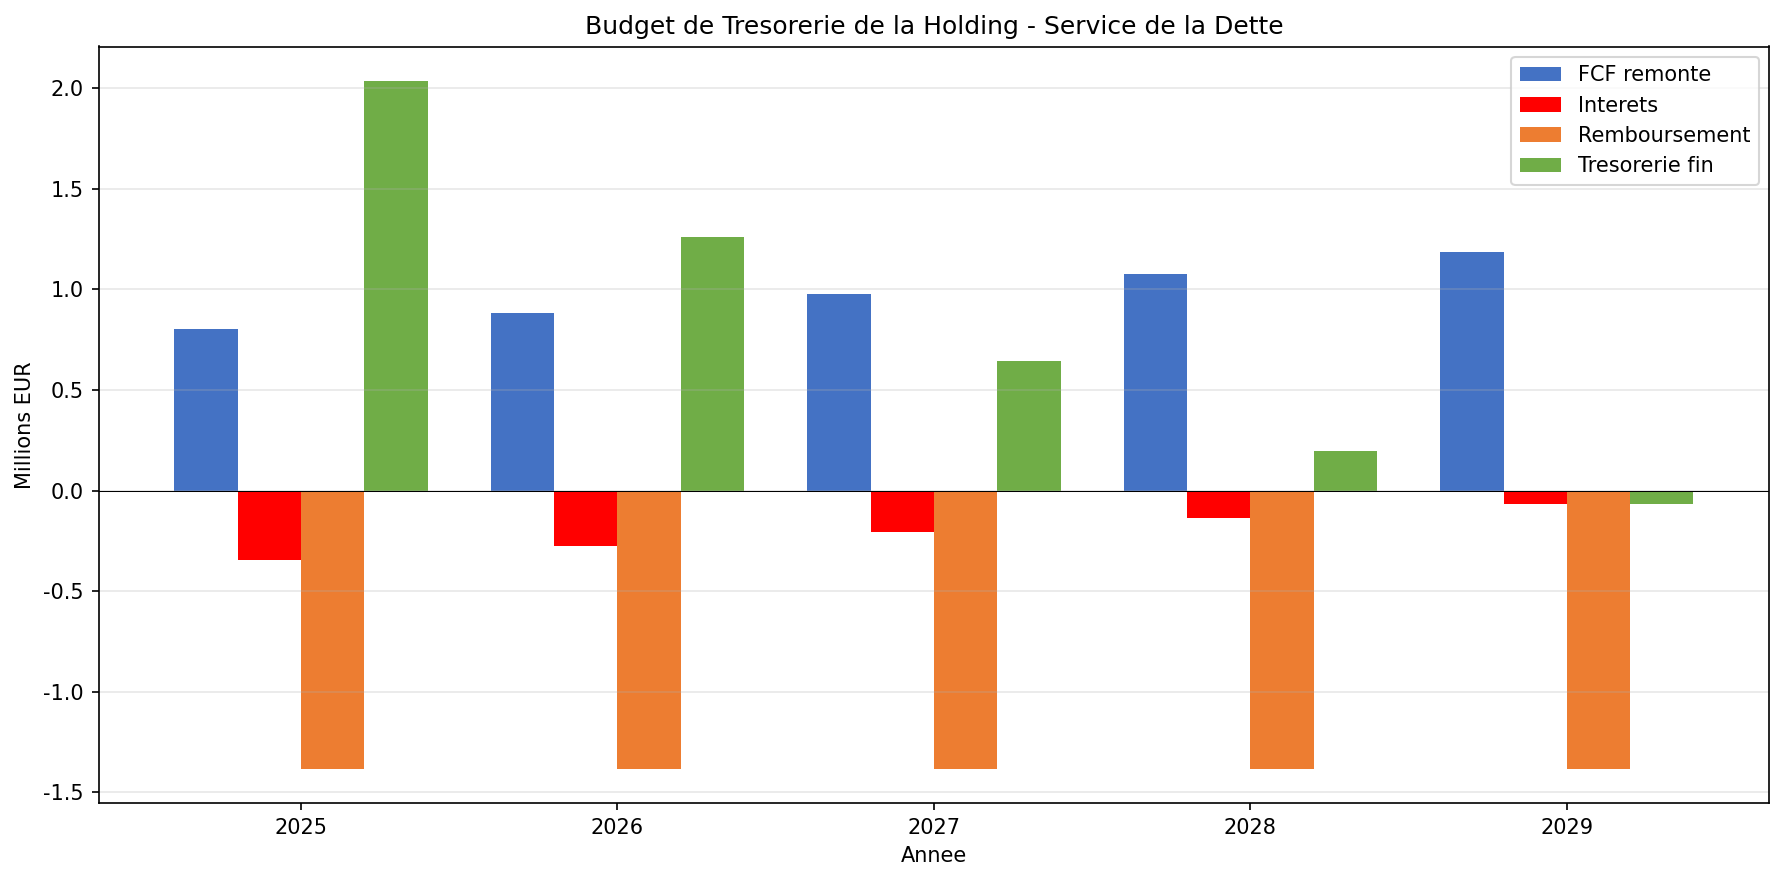
\includegraphics[width=0.7\textwidth]{graphique_budget_tresorerie.png}
\end{figure}

%============================================================
\section{Partie qualitative -- Valorisation des compétences d'ingénieur}
%============================================================

\subsection{Critères de décision pour un investissement significatif}

D'après le cours, les critères déterminants pour lancer un investissement significatif sont :

\begin{enumerate}
    \item \textbf{Valeur Actuelle Nette (VAN)} $> 0$ : l'investissement crée de la valeur
    \item \textbf{Taux de Rentabilité Interne (TRI)} $>$ WACC : la rentabilité dépasse le coût du capital
    \item \textbf{Délai de récupération} (payback) inférieur à 3-4 ans : retour rapide sur investissement
    \item \textbf{Cohérence stratégique} avec le métier de l'entreprise
    \item \textbf{Maîtrise des risques} : analyse de sensibilité aux hypothèses
\end{enumerate}

\subsection{Synthèse des relations Finance / Opérations}

\textbf{Personnes rencontrées (entretiens fictifs)} :
\begin{itemize}
    \item Mme A., Directrice Administrative et Financière
    \item M. B., Contrôleur de gestion
    \item M. C., Responsable logistique (opérations)
\end{itemize}

\textbf{Fréquence des échanges} : réunion mensuelle de pilotage (1h30) + comité d'investissement trimestriel + échanges informels quotidiens.

\textbf{Points de friction identifiés :}
\begin{itemize}
    \item Les opérationnels perçoivent la finance comme un « gendarmes » qui bloque les projets sans comprendre les enjeux techniques.
    \item Les financiers regrettent le manque de rigueur dans les prévisions de coûts et de délais des ingénieurs.
    \item Les indicateurs de performance ne sont pas toujours partagés (trésorerie vs. production).
\end{itemize}

\textbf{Bonnes pratiques mises en place :}
\begin{itemize}
    \item Création d'une fiche projet standardisée intégrant VAN, TRI et analyse de sensibilité.
    \item Reporting mensuel des écarts entre budget et réalisé avec commentaires opérationnels.
    \item Tableau de bord commun (KPIs financiers et opérationnels) accessible à tous.
\end{itemize}

\subsection{Apport de la compréhension des principes financiers pour un ingénieur}

\begin{enumerate}
    \item \textbf{Traduction technique vers économique} : L'ingénieur sait quantifier les gains de productivité, la baisse de consommation énergétique, l'allongement de la durée de vie d'un équipement. La finance transforme ces données en VAN et TRI, langage universel de la direction.
    
    \item \textbf{Dialogue efficace avec la DAF} : Connaître la logique du BFR, du coût du capital ou de l'actualisation permet de présenter les projets dans le format attendu, d'anticiper les objections et de crédibiliser la demande.
    
    \item \textbf{Optimisation globale} : Un ingénieur financièrement formé arbitre entre surdimensionnement technique et rentabilité. Il comprend pourquoi réduire les cycles de production améliore le BFR, ou pourquoi standardiser les composants diminue le besoin en fonds de roulement.
    
    \item \textbf{Leadership et vision} : Dans les comités de direction, parler le même langage que le DAF ou le DG confère une légitimité. L'ingénieur devient un manager capable de défendre ses projets sur le terrain de la création de valeur, pas seulement sur celui de la performance technique.
\end{enumerate}

%============================================================
\section*{Conclusion}
\addcontentsline{toc}{section}{Conclusion}
%============================================================

L'analyse financière de Bricorama France révèle une entreprise saine, peu endettée et rentable. La valorisation DCF aboutit à une valeur d'entreprise de \textbf{67,8 M\text{\euro}} et une valeur des titres de \textbf{60,1 M\text{\euro}}.

Deux montages de financement sont possibles :
\begin{itemize}
    \item \textbf{Cas 1} (dette non consolidée) : Apport minimum de 31,1 M\text{\euro}
    \item \textbf{Cas 2} (dette consolidée) : Apport minimum de 42,0 M\text{\euro}
\end{itemize}

Le cas 2 sécurise davantage le prêteur mais exige plus de fonds propres de la part des investisseurs.

Ce cas pratique illustre parfaitement l'écart entre valeur « mathématique » et valeur « transactionnelle », et souligne l'importance pour l'ingénieur de maîtriser les outils financiers afin de participer activement aux décisions stratégiques.

%============================================================
\section*{Sources}
\addcontentsline{toc}{section}{Sources}
%============================================================

\begin{itemize}
    \item \textcolor{blue}{\texttt{Pappers}} -- Comptes annuels Bricorama France (2022-2024)
    \item \textcolor{blue}{\texttt{Societe.com}} -- Informations légales et bilans
    \item Le Figaro Entreprises -- Données financières
    \item Données de marché du secteur du bricolage en France (FMB)
\end{itemize}

\end{document}